\documentclass[10pt,a4paper]{article}

\usepackage[a4paper,landscape,margin=10mm]{geometry}
\usepackage[T1]{fontenc}
\usepackage{lmodern}
\usepackage{microtype}
\usepackage{xcolor}
\usepackage{enumitem}
\usepackage{tabularx}
\usepackage{tikz}
\usetikzlibrary{arrows.meta,calc,positioning}

\definecolor{ink}{HTML}{172B3A}
\definecolor{navy}{HTML}{164E63}
\definecolor{teal}{HTML}{0F766E}
\definecolor{slate}{HTML}{475569}
\definecolor{line}{HTML}{94A3B8}
\definecolor{paper}{HTML}{FFFFFF}
\definecolor{prepbg}{HTML}{F1F5F9}
\definecolor{sparkbg}{HTML}{ECFEFF}
\definecolor{goldbg}{HTML}{F0FDFA}
\definecolor{oraclebg}{HTML}{F8FAFC}
\definecolor{faultbg}{HTML}{FFF7ED}
\definecolor{fault}{HTML}{C2410C}
\definecolor{quarantine}{HTML}{9F1239}

\pagestyle{empty}
\setlength{\parindent}{0pt}
\setlength{\parskip}{3pt}
\setlist[itemize]{leftmargin=4.2mm,itemsep=2.2pt,topsep=3pt,parsep=0pt}
\setlist[enumerate]{leftmargin=5mm,itemsep=2.5pt,topsep=3pt,parsep=0pt}

\newcommand{\pagetitle}[2]{%
  {\fontsize{20}{23}\selectfont\bfseries\color{ink}#1}\hfill
  {\small\bfseries\color{navy}#2}\par
  \vspace{1mm}\color{line}\rule{\textwidth}{0.6pt}\color{ink}\vspace{2mm}
}

\newcommand{\columnheading}[1]{%
  \colorbox{navy}{\parbox{\dimexpr\linewidth-2\fboxsep\relax}{%
    \color{white}\bfseries\large\strut #1\strut}}\par\vspace{3mm}
}

\begin{document}

\pagetitle{Auditable IoT Energy Data Pipeline}{SYSTEM ARCHITECTURE \quad 1 / 3}

\begin{center}
\colorbox{prepbg}{\parbox{0.965\textwidth}{\centering
\textbf{Research question:} A distributed job has completed. How do we prove
that every delivery was handled correctly and that the resulting decision is
based on independently verified data?}}
\end{center}
\vspace{1mm}

\begin{center}
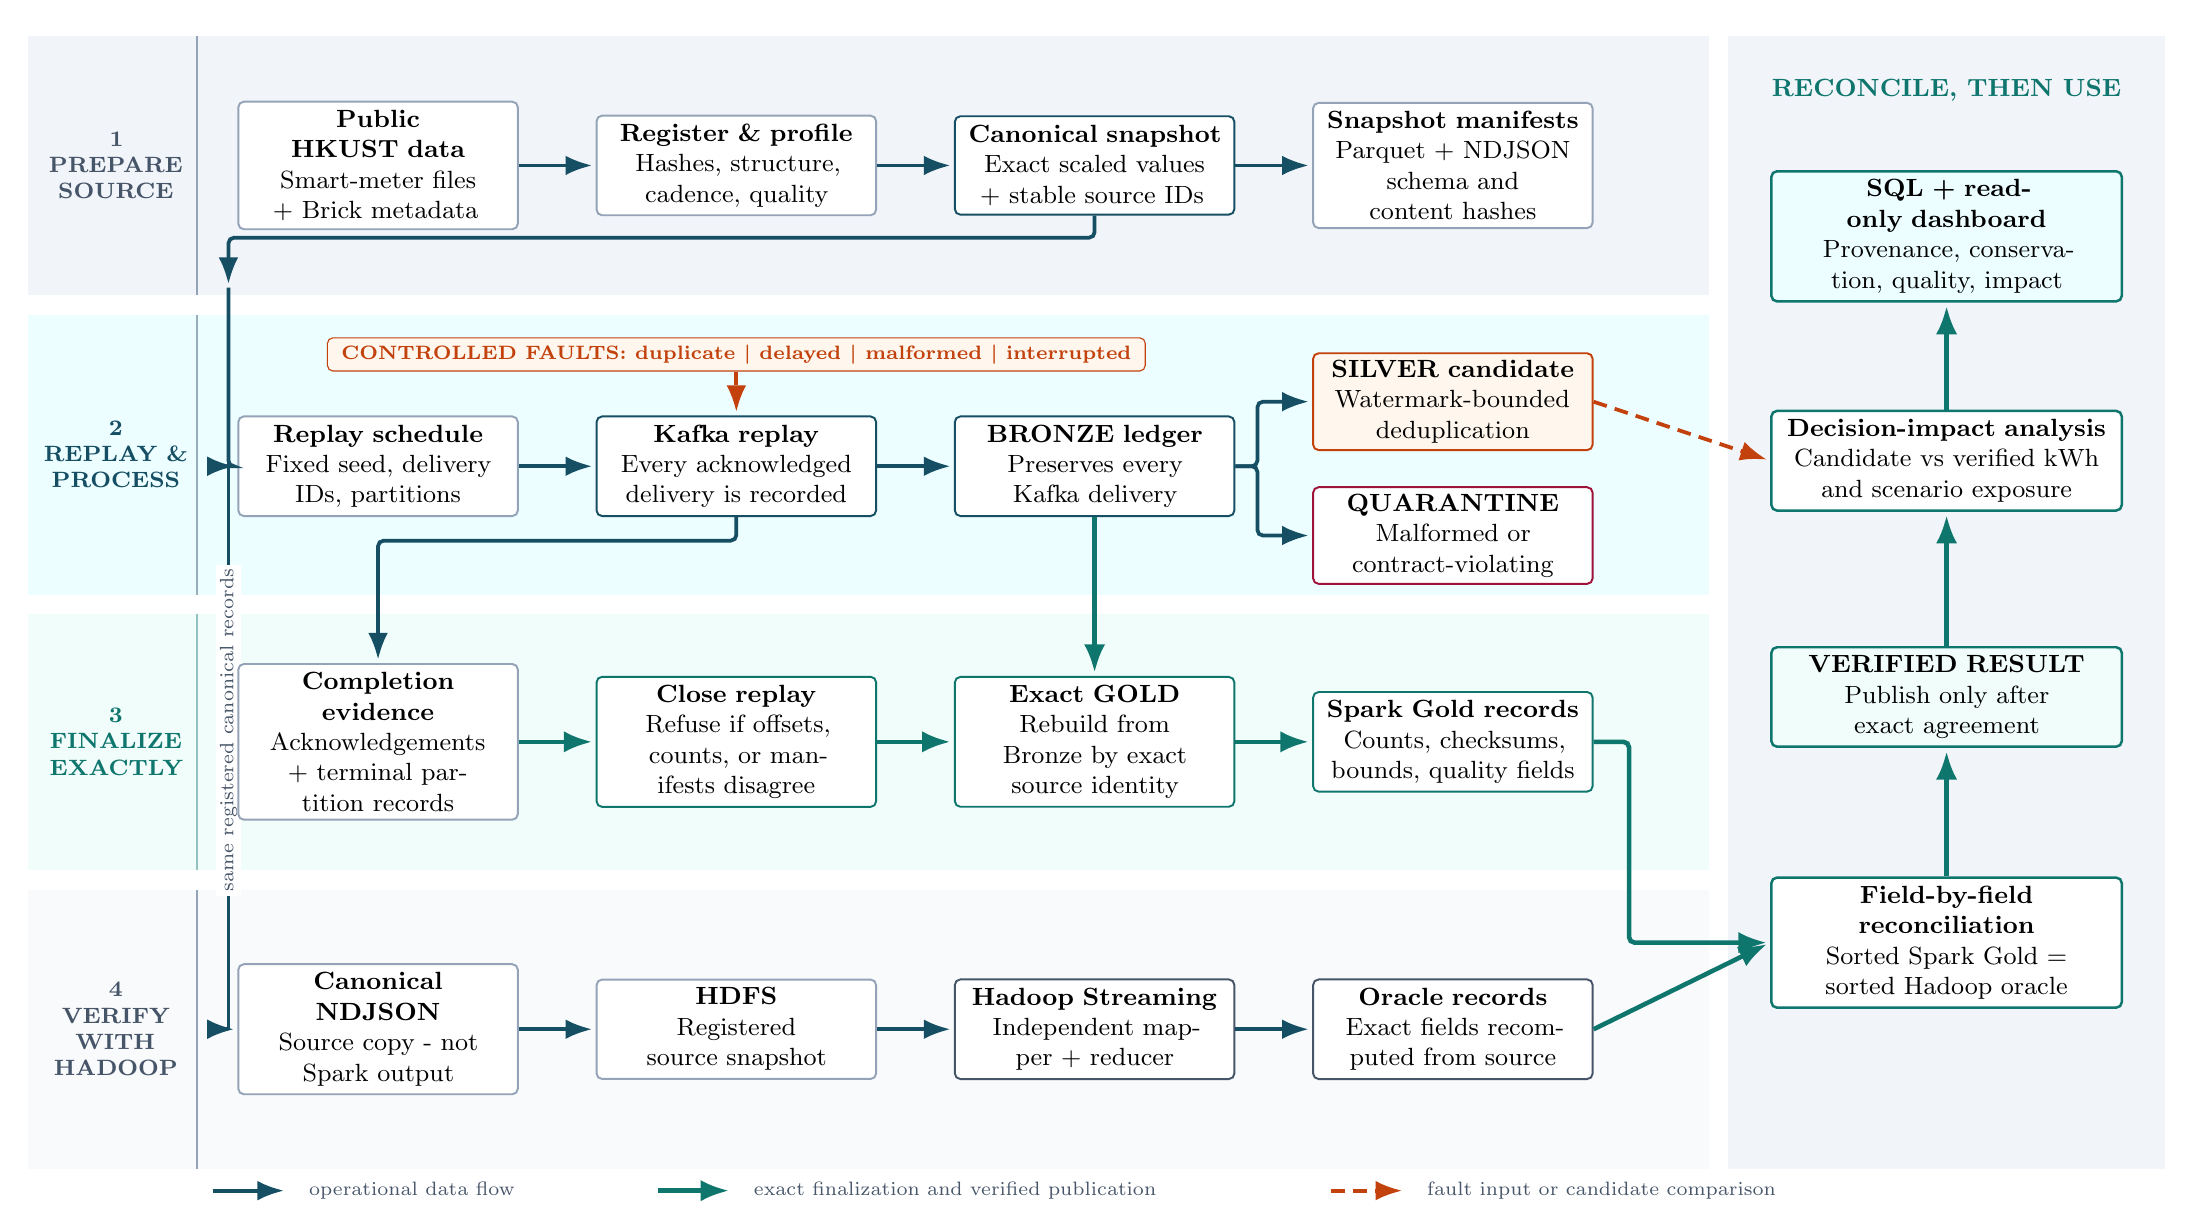
\begin{tikzpicture}[
  x=1cm,
  y=1cm,
  stage/.style={draw=line, fill=paper, rounded corners=2pt, line width=0.7pt,
    align=center, minimum width=3.55cm, minimum height=1.25cm,
    text width=3.2cm, inner sep=3pt, font=\small},
  compact/.style={draw=line, fill=paper, rounded corners=2pt, line width=0.7pt,
    align=center, minimum width=3.55cm, minimum height=1.02cm,
    text width=3.2cm, inner sep=2.5pt, font=\small},
  rightstage/.style={draw=teal, fill=paper, rounded corners=2pt, line width=0.9pt,
    align=center, minimum width=4.45cm, minimum height=1.18cm,
    text width=4.05cm, inner sep=3pt, font=\small},
  lane/.style={align=center, text width=1.85cm, font=\bfseries\footnotesize},
  flow/.style={-{Latex[length=3.4mm,width=2.5mm]}, draw=navy,
    line width=1.35pt, rounded corners=2pt, shorten >=1.2pt},
  verified/.style={-{Latex[length=3.6mm,width=2.7mm]}, draw=teal,
    line width=1.65pt, rounded corners=2pt, shorten >=1.2pt},
  candidate/.style={-{Latex[length=3.4mm,width=2.5mm]}, draw=fault,
    line width=1.35pt, dash pattern=on 5pt off 3pt, rounded corners=2pt,
    shorten >=1.2pt},
  note/.style={font=\scriptsize, text=slate, align=center}
]
  \useasboundingbox (0,0) rectangle (27.2,14.85);

  % Lane backgrounds and labels
  \fill[prepbg]   (0,11.45) rectangle (21.35,14.75);
  \fill[sparkbg]  (0,7.65)  rectangle (21.35,11.20);
  \fill[goldbg]   (0,4.15)  rectangle (21.35,7.40);
  \fill[oraclebg] (0,0.35)  rectangle (21.35,3.90);
  \fill[prepbg]   (21.60,0.35) rectangle (27.15,14.75);

  \node[lane, text=slate] at (1.12,13.10) {1\\PREPARE\\SOURCE};
  \node[lane, text=navy]  at (1.12,9.43)  {2\\REPLAY \&\\PROCESS};
  \node[lane, text=teal]  at (1.12,5.78)  {3\\FINALIZE\\EXACTLY};
  \node[lane, text=slate] at (1.12,2.13)  {4\\VERIFY WITH\\HADOOP};
  \draw[line, line width=0.5pt] (2.15,11.45) -- (2.15,14.75);
  \draw[navy!45, line width=0.5pt] (2.15,7.65) -- (2.15,11.20);
  \draw[teal!45, line width=0.5pt] (2.15,4.15) -- (2.15,7.40);
  \draw[line, line width=0.5pt] (2.15,0.35) -- (2.15,3.90);

  % Source preparation
  \node[stage] (source) at (4.45,13.10)
    {\textbf{Public HKUST data}\\Smart-meter files\\+ Brick metadata};
  \node[stage] (profile) at (9.00,13.10)
    {\textbf{Register \& profile}\\Hashes, structure, cadence, quality};
  \node[stage, draw=navy] (canonical) at (13.55,13.10)
    {\textbf{Canonical snapshot}\\Exact scaled values\\+ stable source IDs};
  \node[stage] (manifest) at (18.10,13.10)
    {\textbf{Snapshot manifests}\\Parquet + NDJSON\\schema and content hashes};
  \draw[flow] (source) -- (profile);
  \draw[flow] (profile) -- (canonical);
  \draw[flow] (canonical) -- (manifest);

  % Canonical-record bus to both computation paths
  \coordinate (busTop) at (2.55,11.55);
  \coordinate (busBottom) at (2.55,2.13);
  \draw[flow] (canonical.south) -- ++(0,-0.28) -| (busTop);
  \draw[draw=navy, line width=1.35pt] (busTop) -- (busBottom);
  \node[note, rotate=90, fill=paper, inner sep=1.5pt] at (2.55,5.93)
    {same registered canonical records};

  % Operational path
  \node[stage] (schedule) at (4.45,9.28)
    {\textbf{Replay schedule}\\Fixed seed, delivery IDs, partitions};
  \node[stage, draw=navy] (kafka) at (9.00,9.28)
    {\textbf{Kafka replay}\\Every acknowledged delivery is recorded};
  \node[stage, draw=navy] (bronze) at (13.55,9.28)
    {\textbf{BRONZE ledger}\\Preserves every Kafka delivery};
  \node[compact, draw=fault, fill=faultbg] (silver) at (18.10,10.10)
    {\textbf{SILVER candidate}\\Watermark-bounded deduplication};
  \node[compact, draw=quarantine] (quar) at (18.10,8.40)
    {\textbf{QUARANTINE}\\Malformed or contract-violating};
  \draw[flow] (busTop) -- (2.55,9.28) -- (schedule.west);
  \draw[flow] (schedule) -- (kafka);
  \draw[flow] (kafka) -- (bronze);
  \draw[flow] (bronze.east) -- ++(0.28,0) |- (silver.west);
  \draw[flow] (bronze.east) -- ++(0.28,0) |- (quar.west);
  \node[draw=fault, fill=faultbg, rounded corners=2pt, text=fault,
    font=\scriptsize\bfseries, inner xsep=5pt, inner ysep=2.5pt]
    (faults) at (9.00,10.70)
    {CONTROLLED FAULTS: duplicate \textbar{} delayed \textbar{} malformed \textbar{} interrupted};
  \draw[candidate] (faults) -- (kafka);

  % Exact finalization path
  \node[stage] (evidence) at (4.45,5.78)
    {\textbf{Completion evidence}\\Acknowledgements + terminal partition records};
  \node[stage, draw=teal] (closegate) at (9.00,5.78)
    {\textbf{Close replay}\\Refuse if offsets, counts, or manifests disagree};
  \node[stage, draw=teal] (gold) at (13.55,5.78)
    {\textbf{Exact GOLD}\\Rebuild from Bronze by exact source identity};
  \node[stage, draw=teal] (goldrecords) at (18.10,5.78)
    {\textbf{Spark Gold records}\\Counts, checksums, bounds, quality fields};
  \draw[flow] (kafka.south) -- ++(0,-0.30) -| (evidence.north);
  \draw[verified] (evidence) -- (closegate);
  \draw[verified] (closegate) -- (gold);
  \draw[verified] (bronze.south) -- (gold.north);
  \draw[verified] (gold) -- (goldrecords);

  % Independent Hadoop path
  \node[stage] (sourcecopy) at (4.45,2.13)
    {\textbf{Canonical NDJSON}\\Source copy - not Spark output};
  \node[stage] (hdfs) at (9.00,2.13)
    {\textbf{HDFS}\\Registered source snapshot};
  \node[stage, draw=slate] (hadoop) at (13.55,2.13)
    {\textbf{Hadoop Streaming}\\Independent mapper + reducer};
  \node[stage, draw=slate] (oracle) at (18.10,2.13)
    {\textbf{Oracle records}\\Exact fields recomputed from source};
  \draw[flow] (busBottom) -- (sourcecopy.west);
  \draw[flow] (sourcecopy) -- (hdfs);
  \draw[flow] (hdfs) -- (hadoop);
  \draw[flow] (hadoop) -- (oracle);

  % Publication and decision path
  \node[font=\bfseries\small, text=teal, align=center] at (24.37,14.05)
    {RECONCILE, THEN USE};
  \node[rightstage] (reconcile) at (24.37,3.23)
    {\textbf{Field-by-field reconciliation}\\Sorted Spark Gold = sorted Hadoop oracle};
  \node[rightstage, fill=goldbg] (verifiedset) at (24.37,6.35)
    {\textbf{VERIFIED RESULT}\\Publish only after exact agreement};
  \node[rightstage] (impact) at (24.37,9.35)
    {\textbf{Decision-impact analysis}\\Candidate vs verified kWh and scenario exposure};
  \node[rightstage, fill=sparkbg] (publish) at (24.37,12.20)
    {\textbf{SQL + read-only dashboard}\\Provenance, conservation, quality, impact};
  \draw[verified] (goldrecords.east) -- ++(0.45,0) |- (reconcile.west);
  \draw[verified] (oracle.east) -- (reconcile.west);
  \draw[verified] (reconcile) -- (verifiedset);
  \draw[verified] (verifiedset) -- (impact);
  \draw[verified] (impact) -- (publish);
  \draw[candidate] (silver.east) -- (impact.west);

  \draw[flow] (2.35,0.08) -- (3.30,0.08);
  \node[note, anchor=west] at (3.45,0.08) {operational data flow};
  \draw[verified] (8.00,0.08) -- (8.95,0.08);
  \node[note, anchor=west] at (9.10,0.08) {exact finalization and verified publication};
  \draw[candidate] (16.55,0.08) -- (17.50,0.08);
  \node[note, anchor=west] at (17.65,0.08) {fault input or candidate comparison};
\end{tikzpicture}
\end{center}

\newpage

\pagetitle{Project Contribution and Research Direction}{CONCISE OVERVIEW \quad 2 / 3}

\begin{center}
\colorbox{prepbg}{\parbox{0.965\textwidth}{\centering\large
\textbf{Core idea:} Completing a Spark job is not proof of data correctness.
The pipeline accounts for every delivery, reconstructs exact results, checks
them through an independently implemented Hadoop computation, and measures the
decision impact of errors that an operational stream may miss.}}
\end{center}
\vspace{2mm}

\begingroup
\small
\setlength{\parskip}{2pt}
\setlist[itemize]{leftmargin=4mm,itemsep=1.1pt,topsep=2pt,parsep=0pt}

\begin{minipage}[t]{0.315\textwidth}
\columnheading{What we are doing}

\textbf{1. Fix the source.}
Register public HKUST smart-meter data and Brick metadata; profile file hashes,
workbook structure, timestamps, cadence, precision, missingness, and duplicate
timestamps.

\textbf{2. Preserve exact identity and value.}
Create deterministic Parquet and NDJSON snapshots. Each row keeps its source
file, sheet, physical row, original text, and decimal value as a scaled integer.

\textbf{3. Replay realistic delivery faults.}
Use fixed seeds to produce clean, duplicate, delayed, malformed, combined, and
interrupted Kafka deliveries. Delivery acknowledgements and terminal partition
records establish what was actually sent.

\textbf{4. Separate operational and final truth.}
Spark Bronze preserves all deliveries. Silver gives a fast,
watermark-bounded candidate; invalid data goes to Quarantine. After replay
completion, Gold is rebuilt exactly from Bronze using source identity.

\textbf{5. Verify before use.}
Hadoop independently recomputes the declared records from canonical NDJSON.
Only reconciled results feed decision-impact reports, SQL queries, and the
read-only dashboard.
\end{minipage}
\hfill
\begin{minipage}[t]{0.315\textwidth}
\columnheading{Why this is novel}

\textbf{The contribution is the combined assurance method, not simply the use
of Kafka, Spark, and Hadoop.}

\begin{itemize}
  \item \textbf{Job success is replaced by conservation evidence.} Every
    source event and acknowledged delivery has a deterministic identity and an
    auditable destination; missing terminals, count mismatches, or manifest
    disagreement prevent finalization.
  \item \textbf{Operational truth and exact truth are explicit.} A bounded
    Silver result is retained as the realistic candidate, while exact Gold is
    rebuilt only after the replay is demonstrably complete.
  \item \textbf{Verification is implementation-diverse.} Hadoop reads the
    registered source rather than Spark output and does not import Spark
    transformation code. Agreement is checked on sorted exact fields.
  \item \textbf{Faults have known ground truth.} Reproducible injection makes
    duplicate handling, late-data behaviour, quarantine, and restart
    equivalence measurable instead of anecdotal.
  \item \textbf{Correctness is connected to decisions.} Candidate-versus-
    verified differences are reported as affected meter-periods, absolute kWh
    discrepancy, and normalized low/base/high billing scenarios.
\end{itemize}
\end{minipage}
\hfill
\begin{minipage}[t]{0.315\textwidth}
\columnheading{Future expansion}

\textbf{If coursework time permits}
\begin{itemize}
  \item Complete the evidence-based real-dataset audit, assigning timezone and
    cumulative-kWh semantics only where the source supports them.
  \item Run the accepted Docker fixture, then designated-machine experiments at
    100K, 1M, and up to 5M/full scale. Measure throughput, recovery, watermarks,
    storage formats, and query performance.
  \item Finalize the generated report, read-only dashboard, and 5-7 minute
    demonstration using prepared results rather than live large workloads.
\end{itemize}

\textbf{Proposed MTP direction}

\textbf{Risk-Adaptive Independent Verification for Decision-Critical IoT Data
Pipelines}

\begin{itemize}
  \item Allocate second-engine verification to high-risk meter-time windows
    using data quality, reset, rollover, gap, metadata, and decision-impact
    signals.
  \item Optimize verification coverage against latency, compute, and storage
    budgets; compare full checking, fixed sampling, and adaptive selection.
  \item Extend to multi-engine oracles, fault localization, online correction,
    and stronger provenance attestations.
  \item Evaluate generalization across buildings, institutions, and additional
    public IoT datasets.
\end{itemize}

\colorbox{goldbg}{\parbox{\dimexpr\linewidth-2\fboxsep\relax}{%
\textbf{MTP research question:} How can a pipeline spend verification effort
where it most reduces expected decision loss while maintaining auditable
correctness under a fixed resource budget?}}
\end{minipage}

\vfill
\begin{tikzpicture}[remember picture,overlay]
  \node[anchor=south west, font=\footnotesize, text=slate]
    at ([xshift=10mm,yshift=6mm]current page.south west) {Nishant Harkut};
  \node[anchor=south, font=\footnotesize, text=slate]
    at ([yshift=6mm]current page.south) {IoT and Big Data Management};
  \node[anchor=south east, font=\footnotesize, text=slate]
    at ([xshift=-10mm,yshift=6mm]current page.south east) {ABV-IIITM Gwalior};
\end{tikzpicture}

\endgroup

\newpage

\pagetitle{What the System Actually Does}{ONE COMPLETE RUN \quad 3 / 3}

\begin{center}
\colorbox{prepbg}{\parbox{0.965\textwidth}{\centering
Follow the numbered central path from source registration to publication. The
left branch is the independent Hadoop check; the right branch preserves the
operational Spark outputs and blocks publication when exact records disagree.}}
\end{center}
\vspace{1mm}

\begin{center}
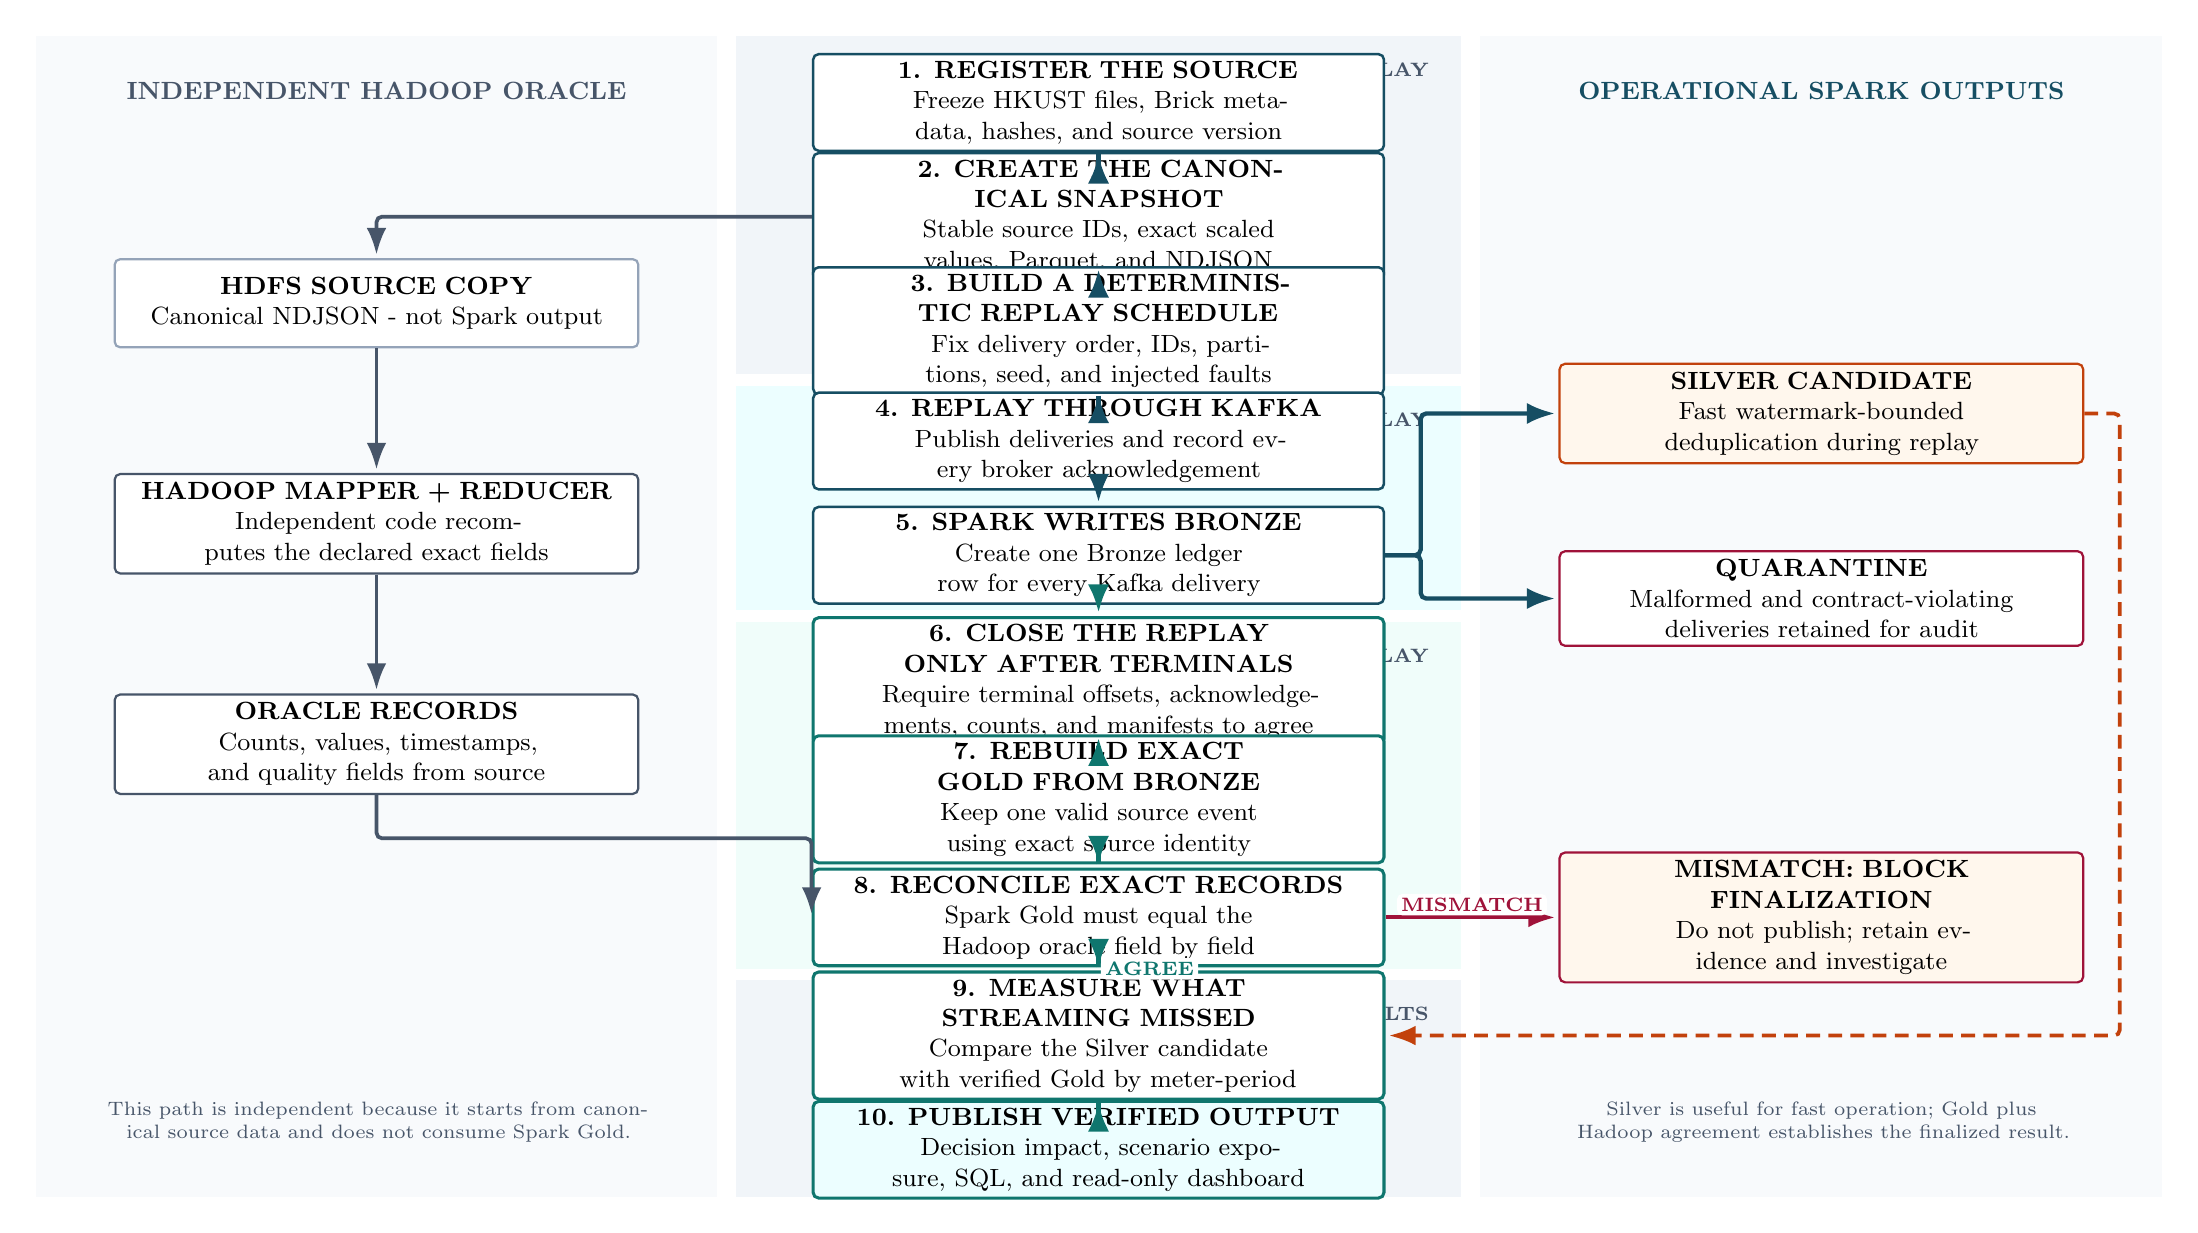
\begin{tikzpicture}[
  x=1cm,
  y=1cm,
  mainstep/.style={draw=navy, fill=paper, rounded corners=2pt,
    line width=0.9pt, align=center, minimum width=7.25cm,
    minimum height=1.02cm, text width=6.75cm, inner sep=2.5pt,
    font=\small},
  exactstep/.style={mainstep, draw=teal, line width=1.1pt},
  side/.style={draw=line, fill=paper, rounded corners=2pt,
    line width=0.8pt, align=center, minimum width=6.65cm,
    minimum height=1.12cm, text width=6.15cm, inner sep=3pt,
    font=\small},
  mainarrow/.style={-{Latex[length=3.6mm,width=2.7mm]}, draw=navy,
    line width=1.55pt, rounded corners=2pt, shorten >=1.2pt},
  exactarrow/.style={-{Latex[length=3.6mm,width=2.7mm]}, draw=teal,
    line width=1.7pt, rounded corners=2pt, shorten >=1.2pt},
  sidearrow/.style={-{Latex[length=3.4mm,width=2.5mm]}, draw=slate,
    line width=1.35pt, rounded corners=2pt, shorten >=1.2pt},
  brancharrow/.style={-{Latex[length=3.4mm,width=2.5mm]}, draw=fault,
    line width=1.35pt, dash pattern=on 5pt off 3pt,
    rounded corners=2pt, shorten >=1.2pt},
  blockarrow/.style={-{Latex[length=3.4mm,width=2.5mm]}, draw=quarantine,
    line width=1.4pt, rounded corners=2pt, shorten >=1.2pt},
  phase/.style={font=\bfseries\scriptsize, text=slate, anchor=north east},
  flowlabel/.style={font=\bfseries\scriptsize, fill=paper, inner sep=1.5pt}
]
  \useasboundingbox (0,0) rectangle (27.2,14.95);

  % Three uncluttered columns: independent check, numbered run, operational outputs.
  \fill[oraclebg] (0.10,0.10) rectangle (8.75,14.85);
  \fill[prepbg]   (9.00,10.55) rectangle (18.20,14.85);
  \fill[sparkbg]  (9.00,7.55)  rectangle (18.20,10.40);
  \fill[goldbg]   (9.00,3.00)  rectangle (18.20,7.40);
  \fill[prepbg]   (9.00,0.10)  rectangle (18.20,2.85);
  \fill[oraclebg] (18.45,0.10) rectangle (27.10,14.85);

  \node[phase] at (17.92,14.62) {BEFORE REPLAY};
  \node[phase] at (17.92,10.18) {DURING REPLAY};
  \node[phase] at (17.92,7.18) {AFTER REPLAY};
  \node[phase] at (17.92,2.63) {USE ONLY VERIFIED RESULTS};

  % Main numbered workflow.
  \node[mainstep] (s1) at (13.60,14.00)
    {\textbf{1. REGISTER THE SOURCE}\\Freeze HKUST files, Brick metadata, hashes, and source version};
  \node[mainstep] (s2) at (13.60,12.55)
    {\textbf{2. CREATE THE CANONICAL SNAPSHOT}\\Stable source IDs, exact scaled values, Parquet, and NDJSON};
  \node[mainstep] (s3) at (13.60,11.10)
    {\textbf{3. BUILD A DETERMINISTIC REPLAY SCHEDULE}\\Fix delivery order, IDs, partitions, seed, and injected faults};
  \node[mainstep] (s4) at (13.60,9.70)
    {\textbf{4. REPLAY THROUGH KAFKA}\\Publish deliveries and record every broker acknowledgement};
  \node[mainstep] (s5) at (13.60,8.25)
    {\textbf{5. SPARK WRITES BRONZE}\\Create one Bronze ledger row for every Kafka delivery};
  \node[exactstep] (s6) at (13.60,6.65)
    {\textbf{6. CLOSE THE REPLAY ONLY AFTER TERMINALS}\\Require terminal offsets, acknowledgements, counts, and manifests to agree};
  \node[exactstep] (s7) at (13.60,5.15)
    {\textbf{7. REBUILD EXACT GOLD FROM BRONZE}\\Keep one valid source event using exact source identity};
  \node[exactstep] (s8) at (13.60,3.65)
    {\textbf{8. RECONCILE EXACT RECORDS}\\Spark Gold must equal the Hadoop oracle field by field};
  \node[exactstep] (s9) at (13.60,2.15)
    {\textbf{9. MEASURE WHAT STREAMING MISSED}\\Compare the Silver candidate with verified Gold by meter-period};
  \node[exactstep, fill=sparkbg] (s10) at (13.60,0.70)
    {\textbf{10. PUBLISH VERIFIED OUTPUT}\\Decision impact, scenario exposure, SQL, and read-only dashboard};

  \draw[mainarrow] (s1) -- (s2);
  \draw[mainarrow] (s2) -- (s3);
  \draw[mainarrow] (s3) -- (s4);
  \draw[mainarrow] (s4) -- (s5);
  \draw[exactarrow] (s5) -- (s6);
  \draw[exactarrow] (s6) -- (s7);
  \draw[exactarrow] (s7) -- (s8);
  \draw[exactarrow] (s8) -- node[right, flowlabel, text=teal] {AGREE} (s9);
  \draw[exactarrow] (s9) -- (s10);

  % Independent computation receives the registered source, never Spark output.
  \node[font=\bfseries\small, text=slate, align=center] at (4.43,14.15)
    {INDEPENDENT HADOOP ORACLE};
  \node[side] (hdfsrun) at (4.43,11.45)
    {\textbf{HDFS SOURCE COPY}\\Canonical NDJSON - not Spark output};
  \node[side, draw=slate] (hadooprun) at (4.43,8.65)
    {\textbf{HADOOP MAPPER + REDUCER}\\Independent code recomputes the declared exact fields};
  \node[side, draw=slate] (oraclerun) at (4.43,5.85)
    {\textbf{ORACLE RECORDS}\\Counts, values, timestamps, and quality fields from source};
  \draw[sidearrow] (s2.west) -- ++(-0.45,0) -| (hdfsrun.north);
  \draw[sidearrow] (hdfsrun) -- (hadooprun);
  \draw[sidearrow] (hadooprun) -- (oraclerun);
  \draw[sidearrow] (oraclerun.south) -- ++(0,-0.55) -| (s8.west);

  % Operational Spark outputs are retained, but only exact agreement can publish.
  \node[font=\bfseries\small, text=navy, align=center] at (22.78,14.15)
    {OPERATIONAL SPARK OUTPUTS};
  \node[side, draw=fault, fill=faultbg] (silverrun) at (22.78,10.05)
    {\textbf{SILVER CANDIDATE}\\Fast watermark-bounded deduplication during replay};
  \node[side, draw=quarantine] (quarrun) at (22.78,7.70)
    {\textbf{QUARANTINE}\\Malformed and contract-violating deliveries retained for audit};
  \node[side, draw=quarantine, fill=faultbg] (blockedrun) at (22.78,3.65)
    {\textbf{MISMATCH: BLOCK FINALIZATION}\\Do not publish; retain evidence and investigate};
  \draw[mainarrow] (s5.east) -- ++(0.45,0) |- (silverrun.west);
  \draw[mainarrow] (s5.east) -- ++(0.45,0) |- (quarrun.west);
  \draw[brancharrow] (silverrun.east) -- ++(0.45,0) |- (s9.east);
  \draw[blockarrow] (s8.east) -- node[above, flowlabel, text=quarantine]
    {MISMATCH} (blockedrun.west);

  \node[font=\scriptsize, text=slate, align=center, text width=7.7cm]
    at (4.43,1.05)
    {This path is independent because it starts from canonical source data and does not consume Spark Gold.};
  \node[font=\scriptsize, text=slate, align=center, text width=7.7cm]
    at (22.78,1.05)
    {Silver is useful for fast operation; Gold plus Hadoop agreement establishes the finalized result.};
\end{tikzpicture}
\end{center}

\end{document}
